\section{Introduction}

\begin{frame}
\frametitle{Terminology}
Classical calculus:
\begin{itemize}
\item \alert{scalar-scalar functions} ($\color{m1}f:\R\rightarrow\R$)
\item scalar-vector functions ($\color{m1}f:\R^d\rightarrow\R$).  
\end{itemize}
Matrix calculus:
\begin{itemize}
\item \alert{scalar-matrix functions} ($\color{m1}f:\R^{m\times
  n}\rightarrow\R$)
\item \alert{matrix-matrix functions}
($\color{m1}f:\R^{m\times
  n}\rightarrow\R^{k\times l}$).
\end{itemize}
Note:
\begin{enumerate}
\item Scalar-matrix derivatives require matrix-matrix derivatives
\item Matrix-matrix derivatives should be computed implicitly
\end{enumerate}
\end{frame}

\begin{frame}
\frametitle{How can we compute the derivative?}
%
\begin{description}
\item[Numerical] Use finite difference formulae for differentiation (e.g.,
%
$\color{m1}
f'(x) \approx \frac{f(x+h)-f(x)}{h}
$
%
). These methods are simple to program, but lose half of all significant
digits.
%
\item[Symbolic] Give the symbolic representation of the derivative without
saying how best to implement the derivative; these are as accurate as they
come.
%
\item[Algorithmic] Something between numeric and symbolic differentiation.
%
The derivative implementation is computed from the code for $\color{m1}f(x)$.
%
\end{description}
%
\end{frame}

\subsection{Numerical Differentiation}
\label{subsec:numeric}

\begin{frame}
\frametitle{Numerical Differentiation}
\framesubtitle{From First-Principles}
%
\colorbox{green!10}{\vbox{
%
\begin{center}
%
Estimate the gradient by looking at the rate of change.
%
\end{center}
%
}}
%
\begin{itemize}
%
\item Finite Difference: $\color{m1} f'(x) \approx \frac{f(x+h)-f(x)}{h} $
%
\item Central Difference: $\color{m1} f'(x) \approx \frac{f(x+h)-f(x-h)}{2h}$
%
\item Imaginary Difference: 
         $\color{m1} f'(x) \approx \mathrm{Im}\left(\frac{f(x+ih)}{h}\right)$
%
\end{itemize}
%
For $\color{m1}h<\epsilon x$, where $\color{m1}\epsilon$ is the machine
precision, these approximations become zero. 
%
Thus $\color{m1}h$ has to be chosen with care.
%
\end{frame}

\begin{frame}
\frametitle{Numerical Differentiation}
\framesubtitle{Imaginary Differentiation Error}
%
The graph shows the error in approximating the derivative for
$\color{m1}f(x)=e^x$ as a function of $\color{m1}h$.
%
\begin{center}
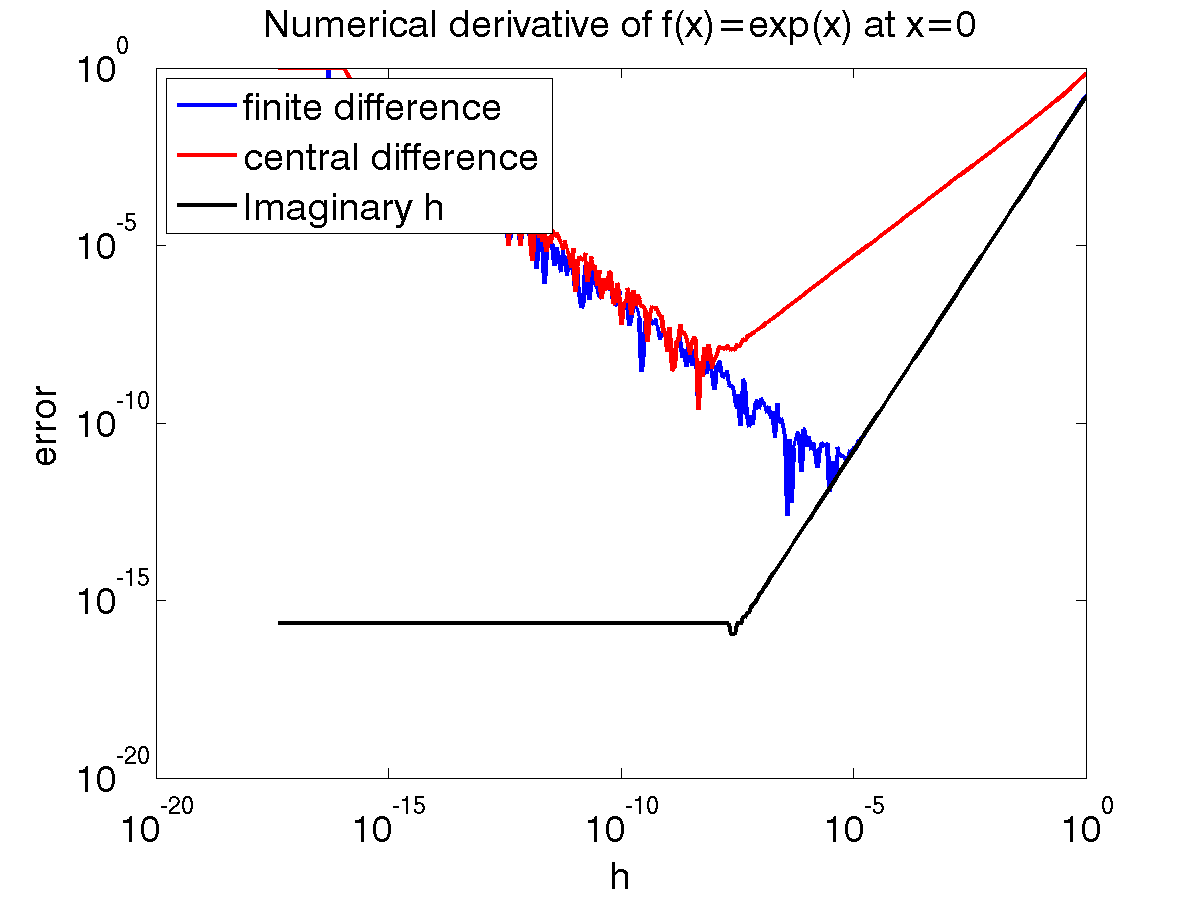
\includegraphics[height=0.5\textwidth]{figs/findifferror2}
\end{center}
%
\end{frame}


\subsection{Symbolic Differentiation}
\label{subsec:symbolic}

\begin{frame}
\frametitle{Symbolic Differentiation}
\framesubtitle{Introduction}
%
\vspace{-20pt}
\begin{center}
\colorbox{green!10}{\vbox{
Calculate derivatives by symbolic manipulation of expressions.
}}
%
\footnotesize
\begin{tabular}{|c|c|}
\hline
Function & \textcolor{blue}{Derivative} \\
\hline
%
$x^p$ & $\color{m1}px^{p-1}$ \\
\hline
$\sin{\theta{}}$ & $\color{m1}\cos{\theta{}}$ \\
\hline
$\cos{\theta{}}$ & $\color{m1}-\sin{\theta{}}$ \\
\hline
$\log{x}$ & $\color{m1}x^{-1}$ \\
\hline
$e^{x}$ & $\color{m1}e^{x}$ \\
\hline
$\frac{d(af(x) + bg(x))}{dx}$ & 
      $\color{m1}a\frac{d(f(x))}{dx} + b\frac{d(g(x))}{dx}$ \\
\hline
$\frac{d(f(x)g(x))}{dx}$ & 
        $\color{m1}f(x)\frac{g(x)}{dx} + g(x)\frac{d(f(x))}{dx}$ \\
\hline
$\frac{d(f(g(x))}{dx}$ & 
        $\color{m1}\frac{d(f(x))}{dg}\frac{d(g(x))}{dx}$ \\
\hline
%
\end{tabular}
\normalsize
%
\end{center}
%
\vspace{-10pt}
\begin{itemize}
\item Minimal set of well-known functions and their derivaties.
\item Rules for computing derivatives of compositions of functions.
\end{itemize}
%
\end{frame}

\begin{frame}
\frametitle{Symbolic Scalar/Vector Differentiation}
%\framesubtitle{Manipulation of identities} 
%
\centerline{$\color{m1}f(x)=x^3;\ f'(x)=3x^2;$}
%
\begin{center}
\begin{minipage}{0.45\textwidth}
\begin{tikzpicture}
[scale=.7,transform shape,
matrix/.style={rectangle,draw=black,fill=blue!20,thick},
operation/.style={circle,draw=black,fill=red!20,thick},
arrow/.style={<-,thick}]

\node[matrix] (x1) {$x$};
\node[matrix, right=2cm of x1] (x2) {$x$};

\node[right=1cm of x1] (x1x2) {};
\node[right=.5cm of x2] (x2x3) {};

\node[operation, above=1.5cm of x1x2] (f1) {$\times{}$} 
edge [arrow] (x2) edge [arrow] (x1);

\node[matrix, right=3cm of f1] (x3) {$x$};
\node[left=0.5cm of x3] (lx3) {};

\node[operation, above=3cm of x2x3] (f2) {$\times{}$}
edge [arrow] (x3) edge [arrow] (f1);

\node[matrix, above=1.2cm of f2] (f) {$f(x)=x^3$} edge [arrow] (f2);

\end{tikzpicture}
\end{minipage}
%
\begin{minipage}{0.45\textwidth}
\begin{tikzpicture}
[scale=.7,transform shape,
matrix/.style={rectangle,draw=black,fill=blue!20,thick},
operation/.style={circle,draw=black,fill=red!20,thick},
arrow/.style={<-,thick}]

\node[matrix] (x1) {$x$};
\node[matrix, right=2cm of x1] (x2) {$3$};

\node[right=1cm of x1] (x1x2) {};
\node[right=.5cm of x2] (x2x3) {};

\node[operation, above=1.5cm of x1x2] (f1) {$\times{}$} 
edge [arrow] (x2) edge [arrow] (x1);

\node[matrix, right=3cm of f1] (x3) {$x$};
\node[left=0.5cm of x3] (lx3) {};

\node[operation, above=3cm of x2x3] (f2) {$\times{}$}
edge [arrow] (x3) edge [arrow] (f1);

\node[matrix, above=1.2cm of f2] (f) {$f'(x)=3x^2$} edge [arrow] (f2);

\end{tikzpicture}
\end{minipage}
\end{center}
\end{frame}

\begin{frame}
\frametitle{Symbolic Differentiation}
\framesubtitle{Drawbacks}
%%
%\footnotesize
%\colorbox{green!10}{\vbox{
%\begin{quote}
%{\color{brown}
%%
%For algebraically rather {\color{blue}simple functions}, the explicit
%derivative expressions obtained by symbolic differentiation may be readable to
%an experienced user and thus provide an {\color{blue}extremely useful
%extension of research} with pencil and paper. However, for functions of any
%{\color{blue}complexity in more than three variables}, the analytic expressions
%for gradient or Hessian tend to take up several pages and are
%{\color{blue}unlikely to facilitate any insights}.
%%
%}\hfill\textbf{\alert{Andreas Grewank}}
%\end{quote}
%}}
%\normalsize
%%
\begin{itemize}
\item Extremely useful for simple functions.
  \begin{itemize}
  \item $\color{m1}f(x)=x^3$.
  \end{itemize}
\item Not helpful for complex functions: may be several pages.
  \begin{itemize}
  \item $\color{m1}
  f(\mSigma)=-\logdet(\mSigma)-\trace(\mS\mSigma^{-1})-\|\mSigma^{-1}\|_F^2$
  \end{itemize}
\item Does not tell us how to compute the derivative.
  \begin{itemize}
  \item Especially because we can reuse computations.
  \end{itemize}
\end{itemize}
\end{frame}



\subsection{Automatic Differentiation}
\label{subsec:automatic}

\begin{frame}
\frametitle{Automatic Differentiation}
\footnotesize
\colorbox{green!10}{\vbox{
\begin{quote}
{\color{brown}
%
Algorithmic/Automatic Differentiation (AD) uses the software representation of
a function to obtain an efficient method for calculating its derivatives.  
%
These derivatives can be of arbitrary order and are analytic in nature (do not
have any truncation error).
}\hfill\textbf{\alert{B. Bell -- author of \texttt{CppAD}}}
\end{quote}
}}
%
\normalsize
\begin{itemize}
  \item No truncation error --- like Symbolic, unlike Numerical.
  \item Gives an algorithm for computing the derivative.
    \begin{itemize}
      \item Often, (conveniently) in terms of the consitituent functions.
    \end{itemize}
\end{itemize}
\end{frame}

%\begin{frame}
%\frametitle{Automatic Scalar Differentiation}
%\framesubtitle{Symbolic Differentiation Comparison}
%
%\begin{center}
%\vspace{-40pt}
%\colorbox{green!10}{\vbox{
%Algorithmic $\approx$ Symbolic, but is more suited for computers as it gives
%an algorithm to compute the derivate.
%}}
%\end{center}
%%
%Consider the function $\color{m1}f(x)=x^3$
%%
%\begin{itemize}
%  \item Symbolic: we apply the power rule to get $\color{m1}f(x)=3x^2$
%  \item Algorithmic: we see $\color{m1}f(x)$ as $\color{m1}=g(g(x,x),x)$
%    \tiny
%    \begin{enumerate}
%      \item %Product/chain rule: 
%        $\color{m1}f'(x)=g\left(\frac{d(g(x,x))}{dx},x\right) + 
%                         g\left(\frac{dx}{dx},g(x,x)\right)$
%      \item %Product/chain rule: 
%        $\color{m1}f'(x)=g\left(g\left(x,\frac{dx}{dx}\right)+
%                                g\left(\frac{dx}{dx},x\right),x\right) + 
%                         g\left(\frac{dx}{dx},g\left(x,x\right)\right)$
%      \item %Reduction: 
%        $\color{m1}f'(x)=g\left(g\left(x,1\right)+
%                         g\left(1,x\right),x\right) + 
%                         g\left(1,g\left(x,x\right)\right)$
%      \item %Reduction: 
%        $\color{m1}f'(x)=(x+x)*x + x^2 = 2x^2 + x^2 = 3x^2$
%    \end{enumerate}
%    \normalsize
%\end{itemize}
%\end{frame}

\begin{frame}
\frametitle{Automatic Scalar/Vector Differentiation}
\framesubtitle{Forward and Reverse Mode} 
%
\centerline{Compute $\color{m1}f'(x); f(x)=x^3$}
%
\begin{center}
\begin{tikzpicture}
[scale=.7,transform shape,
matrix/.style={rectangle,draw=black,fill=blue!20,thick},
operation/.style={circle,draw=black,fill=red!20,thick},
arrow/.style={<-,thick}]

\node[matrix] (x1) {$x$};
\node[matrix, right=2cm of x1] (x2) {$x$};

\node[left=0.5cm of x1] (lx1) {};
\node[left=0.5cm of x2] (lx2) {};

\node[right=1cm of x1] (x1x2) {};
\node[right=.5cm of x2] (x2x3) {};

\node[operation, above=1.5cm of x1x2] (f1) {$\times{}$} 
edge [arrow] (x2) edge [arrow] (x1);

\node[matrix, right=3cm of f1] (x3) {$x$};
\node[left=0.5cm of x3] (lx3) {};

\node[operation, above=3cm of x2x3] (f2) {$\times{}$}
edge [arrow] (x3) edge [arrow] (f1);

\node[matrix, above=1.2cm of f2] (f) {$f(x)=x^3$} edge [arrow] (f2);

\node[left,align=center] (textf1) at (f1.west){$\color{blue}t_1=x^2$};
\node[left,align=center] (textf2) at (f2.west){$\color{blue}t_2=xt_1$};
\node[left,align=center] (textf) at (f.west) {$\color{blue}f=t_2$};

\onslide<2-5>{
\node[left,align=center] (textx1) at (x1.west) {$\color{red}1$};
\node[left,align=center] (textx2) at (x2.west) {$\color{red}1$};
\node[left,align=center] (textx3) at (x3.west) {$\color{red}1$};
}
\onslide<3-5>{
\node[above=1.5pt of textf1, align=center] (textd1) 
                                          {$\color{red}t_1'=x+x$};
}
\onslide<4-5>{
\node[above=1.5pt of textf2, align=center] (textd2)
                                          {$\color{red}t_2'=xt_1'+t_1$};
}
\onslide<5>{
  \node[above=1.2pt of textf,align=center] (textd) {$\color{red}f'=t_2'$};
}

\onslide<6>{
  \node[above=1.2pt of textf,align=center] (textr) 
            {$\color{magenta}r=0, i=1$};
}
\onslide<7-10>{
\node[above=1.2pt of textf2,align=center] (textr2) 
                                  {$\color{magenta}r=0,i=1$};
}
\onslide<8-10>{
\node[above=1.2pt of textf1,align=center] (textr1) 
                                  {$\color{magenta}r=0,i=x$};
}
\onslide<8>{
\node[right=0.2cm of x3] (textr3) {$\color{magenta}r=0,i=t_1$};
}

\onslide<9>{
\node[left=0.2cm of x1] (textr1) {$\color{magenta}r=0,i=x^2$};
\node[right=0.2cm of x2] (textr2) {$\color{magenta}r=0,i=x^2$};
\node[right=0.2cm of x3] (textr3) {$\color{cyan}r=t_1$};
}

\onslide<10>{
\node[left=0.2cm of x1] (textr1) {$\color{cyan}r=x^2$};
\node[right=0.2cm of x2] (textr2) {$\color{cyan}r=x^2$};
\node[right=0.2cm of x3] (textr3) {$\color{cyan}r=x^2$};
}

\end{tikzpicture}

\onslide<2-5>{\begin{center}\textcolor{blue}
                    {Forward Mode: Inside-out Application}\end{center}}
\vspace{-30pt}
\onslide<6-10>{\begin{center}\textcolor{magenta}
                    {Reverse Mode: Outside-in Application}\end{center}}

\end{center}
\end{frame}

\begin{frame}
\frametitle{Automatic Scalar/Vector Differentiation}
\framesubtitle{Notes on Reverse Mode Differentiation}
%
Reverse Mode Differentiation (1971):
%
\begin{itemize}
  \item Chain rule applied in reverse order of function evaluation.
  \item Same technique as:
    \begin{itemize}
      \item Back-propagation algorithm (1969) for neural networks.
      \item Forward-backward algorithm for training HMMs (1970).
    \end{itemize}
  \item Applies to very general classes of functions.
\end{itemize}
%
\end{frame}

\begin{frame}
\frametitle{Automatic Scalar/Vector Differentiation}
\framesubtitle{Computational Cost of Differentiation}
\colorbox{green!10}{\vbox{
\begin{quote}
{\color{brown}Under quite realistic assumptions the evaluation of a gradient
requires never more than five times the effort of evaluating the
underlying function by itself.}\\
\hfill\textbf{\alert{Andreas Griewank (1988)}}
\end{quote}
}}
\end{frame}


\subsection{Scalar-Matrix Derivatives}
\label{subsec:scalar_matrix_diff}

\begin{frame}
\frametitle{Scalar-Matrix Derivatives}
\framesubtitle{Definition}
%
\begin{center}
\vspace{-40pt}
\colorbox{green!10}{\vbox{
Derivative is the rate of change of $\color{m1}f(\mX)$ w.r.t each 
$\color{m1}x_{ij}$
}}
\end{center}

For $\color{m1}f:\R^{m\times n}\rightarrow\R$ the scalar-matrix derivative is
defined to be: 
$$\color{m1}
\frac{\partial f}{\partial \mX} \stackrel{\mathrm{def}}{=} 
\begin{pmatrix} 
\frac{\partial f}{\partial {x_{11}}} &
\frac{\partial f}{\partial {x_{12}}} & \cdots & 
\frac{\partial f}{\partial {x_{1n}}}\\
\frac{\partial f}{\partial x_{21}} &
\frac{\partial f}{\partial x_{22}} & \cdots & 
\frac{\partial f}{\partial x_{2n}}\\
\vdots & \vdots & \ddots & \vdots \\
\frac{\partial f}{\partial x_{m1}} &
\frac{\partial f}{\partial x_{m2}} & \cdots & 
\frac{\partial f}{\partial x_{mn}}
\end{pmatrix}.
$$
\end{frame}

\begin{frame}
\frametitle{Scalar-Matrix Derivatives}
\framesubtitle{Derivative of $\trace \mX$}
%
\begin{center}
\colorbox{green!10}{\vbox{
Derivative is the rate of change of $\color{m1}f(\mX)$ w.r.t each 
$\color{m1}x_{ij}$
}}
\end{center}
%
\textcolor{blue}{
\begin{align*}
f(\mX) &= \trace 
\begin{pmatrix} 
  x_{11} & x_{12} \\
  x_{21} & x_{22} 
\end{pmatrix}  \\
f'(\mX) &= 
\begin{pmatrix} 
  \frac{\partial(x_{11}+x_{22})}{\partial x_{11}} & 
  \frac{\partial(x_{11}+x_{22})}{\partial x_{12}}  \\
  \frac{\partial(x_{11}+x_{22})}{\partial x_{21}} & 
  \frac{\partial(x_{11}+x_{22})}{\partial x_{22}}  \\
\end{pmatrix}   \\
&=
\begin{pmatrix} 
  1 & 0 \\
  0 & 1 
\end{pmatrix} \\
&= \mI
\end{align*}
} % textcolor
\end{frame}

\begin{frame}
\frametitle{Scalar-Matrix Derivatives}
\framesubtitle{Derivative of $\logdet \mX$}
%
\begin{center}
\colorbox{green!10}{\vbox{
Derivative is the rate of change of $\color{m1}f(\mX)$ w.r.t each 
$\color{m1}x_{ij}$
}}
\vspace{-20pt}
\end{center}
\textcolor{blue}{
\footnotesize
\begin{align*}
f(\mX) &= \logdet 
\begin{pmatrix} 
  x_{11} & x_{12} \\
  x_{21} & x_{22} 
\end{pmatrix} \\
f'(\mX) &= 
\begin{pmatrix} 
  \frac{\partial (\log x_{11}x_{22}-x_{12}x_{21})}{\partial x_{11}} & 
  \frac{\partial (\log x_{11}x_{22}-x_{12}x_{21})}{\partial x_{12}}  \\
  \frac{\partial (\log x_{11}x_{22}-x_{12}x_{21})}{\partial x_{21}} & 
  \frac{\partial (\log x_{11}x_{22}-x_{12}x_{21})}{\partial x_{22}}  \\
\end{pmatrix} \\ 
&= \frac{1}{x_{11}x_{22}-x_{12}x_{21}}
\begin{pmatrix} 
  \frac{\partial(x_{11}x_{22}-x_{12}x_{21})}{\partial x_{11}} & 
  \frac{\partial(x_{11}x_{22}-x_{12}x_{21})}{\partial x_{12}}  \\
  \frac{\partial(x_{11}x_{22}-x_{12}x_{21})}{\partial x_{21}} & 
  \frac{\partial(x_{11}x_{22}-x_{12}x_{21})}{\partial x_{22}}  \\
\end{pmatrix}  \\
&= \frac{1}{\det \mX}
\begin{pmatrix} 
  x_{22} & -x_{21}  \\ 
  -x_{12} &  x_{11}  \\ 
\end{pmatrix}  \\
&= \mX^{-\!\top}
\end{align*}
} % textcolor
\normalsize
%
\end{frame}


\subsection{Matrix-Matrix Derivatives}
\label{subsec:mat_mat_diff}

\begin{frame}
\frametitle{Matrix-Matrix Derivatives}
\framesubtitle{Why}
%
\begin{center}
\vspace{-40pt}
\colorbox{green!10}{\vbox{
Derivative is the rate of change of $\color{m1}\mF(\mX)$ w.r.t each 
$\color{m1}x_{ij}$
}}
\end{center}
%
Scalar-matrix derivative of $\color{m1}f(\mG(\mX))$ requires
the information in the matrix-matrix derivative $\color{m1}
\frac{\partial\mG}{\partial\mX}$. For example:

\begin{itemize}
  \item 
    $\color{m1} \trace \left(\left(\left(\mI+\mX\right)^{-1}\right)\mX\right)$
\end{itemize}
%
\begin{center}
Desiderata: The derivative of a matrix-matrix function should be a matrix, so
that a convenient chain-rule can be established.
\end{center}
%
\end{frame}

\begin{frame}
\frametitle{Matrix-Matrix Derivative}
\framesubtitle{The Arrangement Problem}
%
\begin{itemize}
\item For 
  $\color{m1}\mF(\mX)=\mY; \mX\in{}\R^{m\times{}n}, \mY\in{}\R^{k\times{}l},
  \mF'(\mX) \in{} \R^{mn\times{}kl}$
  \begin{itemize}
    \item $\color{m1}\mF'(\mX)$ is a 4-D structure.
    \item How do you represent $\color{m1}\mF'(\mX)$ in 2-D?
  \end{itemize}
\end{itemize}
%
\vspace{-20pt}
\textcolor{blue}{
\begin{align*}
\mF(\mX) &= \mX \\
\mF'
\begin{pmatrix} 
  x_{11} & x_{12} \\
  x_{21} & x_{22} 
\end{pmatrix}
&=
\begin{pmatrix}
\begin{pmatrix} 1 & 0 \\ 0 & 0 \end{pmatrix} &
\begin{pmatrix} 0 & 1 \\ 0 & 0 \end{pmatrix} \\
\begin{pmatrix} 0 & 0 \\ 1 & 0 \end{pmatrix} &
\begin{pmatrix} 0 & 0 \\ 0 & 1 \end{pmatrix} \\
\end{pmatrix}
\end{align*}
} % textcolor
\vspace{-20pt}
%
\begin{center}
  \textcolor{red}{$\mF'(\mX)$ does not have nice structure\!}
\end{center}
%
\end{frame}

\begin{frame}
\frametitle{Matrix-Matrix Derivatives}
\framesubtitle{The vec Operator}
%
\begin{center}
For $\color{m1}\mA\in \R^{m\times n}$, $\color{m1} \myvec(\mA)$  is the
column-stacked vector of $\color{m1}\mA$
\end{center}
%
$$\color{m1}
\myvec(\mA) = 
\begin{pmatrix} 
a_{11} \\
a_{21} \\
\vdots \\
a_{m1} \\
a_{12} \\
\vdots \\
a_{mn} \\
\end{pmatrix}
$$
\end{frame}

\begin{frame}
\frametitle{The Matrix-Matrix Derivative}
\framesubtitle{Definition}
%
We define the matrix--matrix derivative to be: 
%
$$\color{m1}
\frac{\partial \mF}{\partial \mX} \stackrel{\mathrm{def}}{=} 
\frac{\partial
  \myvec(\mF^\top)}{\partial \myvec^\top(\mX^\top)} = 
\begin{pmatrix} 
\frac{\partial \alert<3>{f_{11}}}{\partial \alert<2>{x_{11}}} &
\frac{\partial f_{11}}{\partial \alert<2>{x_{12}}} & \cdots & 
\frac{\partial f_{11}}{\partial \alert<2>{x_{mn}}}\\
\frac{\partial \alert<3>{f_{12}}}{\partial x_{11}} &
\frac{\partial f_{12}}{\partial x_{12}} & \cdots & 
\frac{\partial f_{12}}{\partial x_{mn}}\\
\vdots & \vdots & \ddots & \vdots \\
\frac{\partial \alert<3>{f_{kl}}}{\partial x_{11}} &
\frac{\partial f_{kl}}{\partial x_{12}} & \cdots & 
\frac{\partial f_{kl}}{\partial x_{mn}}
\end{pmatrix}.
$$
%\onslide<4>{
%Caveat: The matrix--matrix derivative of a scalar--matrix function
%is not the same as the scalar--matrix derivative:
%$$\color{m1}
%\frac{\partial\;\mbox{mat}(f)}{\partial\mX} = \myvec^\top\left(
%\left( \frac{\partial f}{\partial\mX}\right)^\top
%\right) .
%$$}
\begin{itemize}
\item This rule seems arcane at first.
\begin{itemize}
\item Results derivatives being well-behaved matrices.
\end{itemize}
\end{itemize}
\end{frame}

\begin{frame}
\frametitle{Matrix-Matrix Derivative}
\framesubtitle{The Arrangement Problem ($\mF(\mX) = \mX$)}
%
\footnotesize
\textcolor{blue}{
\begin{align*}
\mF'
\begin{pmatrix} 
  x_{11} & x_{12} \\
  x_{21} & x_{22} 
\end{pmatrix}
=
\frac{\partial \myvec(\mF^\top)}{\partial \myvec^\top(\mX^\top)}
&= 
\frac{\begin{pmatrix} x_{11} \\ x_{12} \\ x_{21} \\ x_{22} \end{pmatrix}}
{\begin{pmatrix} x_{11} & x_{12} & x_{21} & x_{22} \end{pmatrix}} \\
%
&= 
\begin{pmatrix} 
  1 & 0 & 0 & 0 \\
  0 & 1 & 0 & 0 \\
  0 & 0 & 1 & 0 \\
  0 & 0 & 0 & 1 \\
\end{pmatrix} \\
&= \mI_{d^2\times{}d^2} \\
&= \mI_{d\times{}d}\otimes{}\mI_{d\times{}d}
\end{align*}
} % textcolor
\normalsize
\end{frame}

\subsection{Direct Matrix Products}
%
\begin{frame}
\frametitle{Direct Matrix Products}
\framesubtitle{Derivatives of \emph{Linear} Matrix-Matrix Functions}
%
\begin{enumerate}
\item A matrix--matrix derivative is a matrix outer-product:
$$\color{m1} F(\mX) = \trace(\mA\mX)\mB,\qquad\frac{\partial
    F}{\partial\mX} = \myvec(\mB^\top)\myvec^\top(\mA).
$$
\item A matrix--matrix derivative is a Kronecker product:
$$\color{m1} F(\mX) = \mA\mX\mB,\qquad\frac{\partial
    F}{\partial\mX} = \mA\otimes\mB^\top.
$$
\item A matrix--matrix derivative \alert{box product}.
$$\color{m1} F(\mX) = \mA\mX^\top\mB,\qquad\frac{\partial
    F}{\partial\mX} = \mA\alert{\boxtimes}\mB^\top.
$$
\end{enumerate}
\end{frame}

\begin{frame}
\frametitle{Matrix-Matrix Derivatives}
\framesubtitle{Direct Matrix Products}
%
\alert{Direct Matrix Product}, $\color{m1}\mX=\mA\circledast\mB$, is
a matrix such that:
$$\color{m1}
x_{(i_1i_2)(i_3i_4)}=a_{i_{\sigma(1)}i_{\sigma(2)}}b_{i_{\sigma(3)}i_{\sigma(4)}}.
$$ 
\vspace{-.5cm}

\begin{itemize}
\item $\color{m1}(i_1i_2)$ is shorthand for $\color{m1}i_1n_2+i_2-1$
  where $\color{m1}i_2\in\{1,2,\ldots,n_2\}$.
\item  $\color{m1}\sigma$ is a permutation over $\color{m1}\mathbb{Z}_4$
\end{itemize}
%
\begin{center}
  There are 24 possible permutations that can occur
\end{center}
%
\end{frame}

\begin{frame}
\frametitle{Matrix-Matrix Derivatives}
\framesubtitle{Direct Matrix Product}
%
\begin{itemize}
  \item 8 can be expressed using matrix outer products.
$$
\scriptsize
\color{m1}
\begin{array}{cccc}
  \myvec(\mA)\myvec(\mB)^\top & \myvec(\mA^\top) \myvec(\mB)^\top &
  \myvec(\mB)\myvec(\mA)^\top & \myvec(\mB^\top) \myvec(\mA)^\top \\
  \myvec(\mA)\myvec(\mB^\top)^\top & \myvec(\mA^\top) \myvec(\mB^\top)^\top &
  \myvec(\mB)\myvec(\mA^\top)^\top & \myvec(\mB^\top) \myvec(\mA^\top)^\top \\
\end{array}
$$
\normalsize
  \item 8 can be expressed using Kronecker products.
\footnotesize
$$
\color{m1}
\begin{array}{cccc}
\mA\otimes\mB     & \mA^\top\otimes\mB &
\mA\otimes\mB^\top & \mA^\top\otimes\mB^\top \\
\mB\otimes\mA     & \mB^\top\otimes\mA &
\mB\otimes\mA^\top & \mB^\top\otimes\mA^\top
\end{array}
$$
\normalsize
\textcolor{red}{
  \item Remaining 8 can be expressed using Box products.
\footnotesize
$$
\begin{array}{cccc}
\mA\boxtimes\mB     & \mA^\top\boxtimes\mB &
\mA\boxtimes\mB^\top & \mA^\top\boxtimes\mB^\top \\
\mB\boxtimes\mA     & \mB^\top\boxtimes\mA &
\mB\boxtimes\mA^\top & \mB^\top\boxtimes\mA^\top
\end{array}
$$
} % textcolor
\normalsize
\end{itemize}
%
\end{frame}


